\chapter{Black-Box Optimization}

One of the most exciting challenges in the optimization practice is the possibility to optimize in absence of an explicit algebraic model of the system to be optimized. This kind of optimization is known as \textit{black-box optimization} and it is the subject matter of this dissertation. \\

A black-box function $f(x) : \mathbb{R}^n \rightarrow \mathbb{R}$ is a function for which the analytic form is not known. Nowadays there are lots of mathematical models to succeed in optimize this kind of functions. One of the best known of these methods is the \textit{Bayesian Optimization} (BO) typically based on \textit{Gaussian Processes} (GPs) as probabilistic surrogate model. \\

In this chapter the BO model will be analysed and then an innovative, Reinforcement Learning  based approach to solve the same problem will be proposed.

\subsection{Gaussian Processes} Before introducing BO it is necessary to describe what \textit{Gaussian Processes} (GPs) are. GPs are an alternative approach to regression problems. GPs are a \textit{non-parametric} approach (there is not a priori knowledge of how many parameters will be useful for the regression) to find a distribution over the possible functions $f(x)$ that are consistent with observed data. A GP is a generalization of the Gaussian probability distribution. Whereas a probability distribution describes random variables which are scalars or vectors (for multivariate distributions), a \textit{stochastic process} governs the properties of functions. \\

GP is a convenient and powerful prior distribution on functions, which will be taken here to be of the form 

\begin{equation}
	f : \mathcal{X} \leftarrow \mathbb{R}.
\end{equation}

The GP is defined by the property that any finite set of $N$ points $\{x_n \in \mathcal{X}\}\subsup{}{ n=1}{N}$ induces a multivariate Gaussian distribution  on $\mathbb{R}^N$. The $n$\textsuperscript{th} of those points is taken to be the function value $f(x_n)$~\cite{NIPS2012_4522}. The support and properties of the resulting distribution on functions are determined by a mean function 

\begin{equation}
	m : \mathcal{X} \leftarrow \mathbb{R}
\end{equation}

and by a positive definite covariance function 

\begin{equation}
	k : \mathcal{X} \times \mathcal{X} \leftarrow \mathbb{R}.
\end{equation}

\begin{figure} [h!]
	\centering
	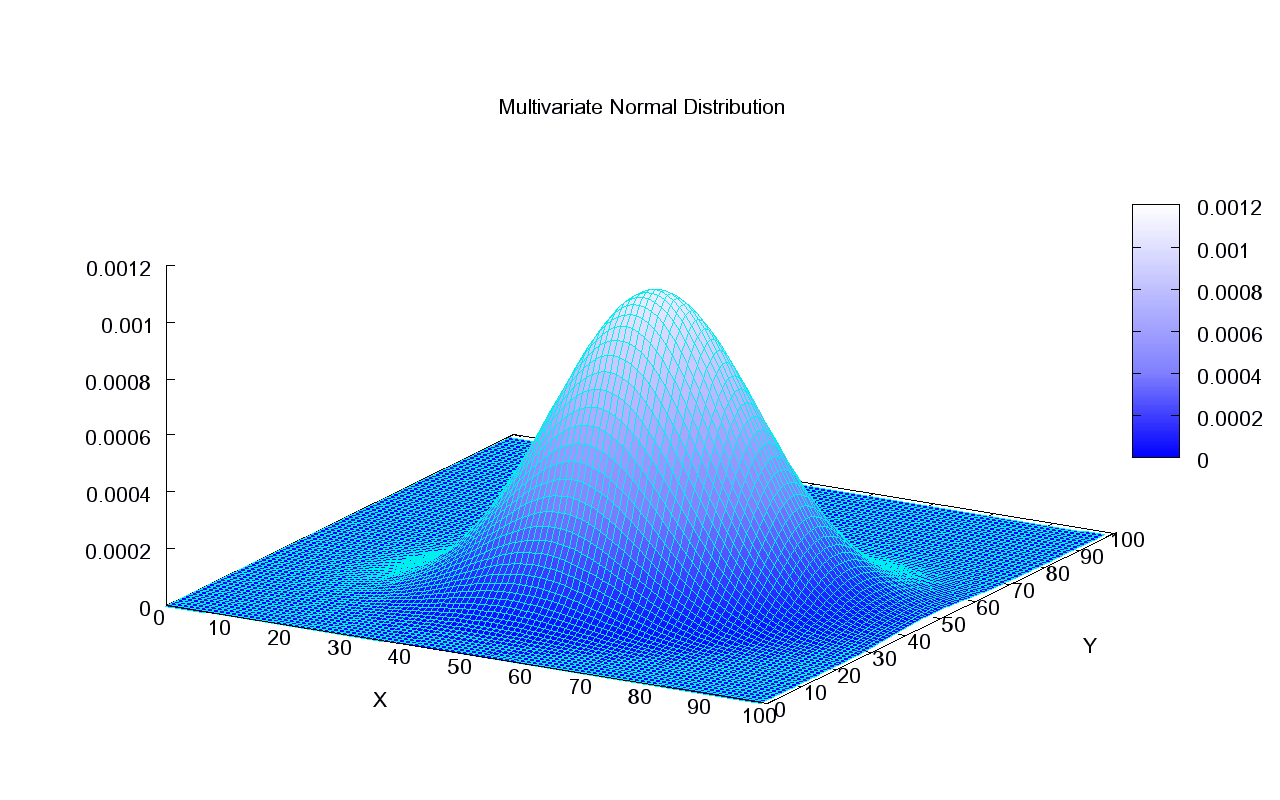
\includegraphics[width= \textwidth, height = 8cm]{Multivariate_Gaussian.png}
	\caption{Multivariate Gaussian Distribution~\cite{MNDWikipedia}.}
	\label{fig:Multivatiate_Gaussian}
\end{figure}

\subsection{Bayesian Optimization} Let's assume that the function $f(x)$ is drawn from a GP prior and that observations are of the form $\{x_n \in \mathcal{X}\}\subsup{}{ n=1}{N}$, with $y_n \sim \mathcal{N}(f(x_n), v)$ where $v$ is the variance of noise introduced into the function observations. This prior and those data induce  posterior over functions; the acquisition function, which is denoted by

\begin{equation}
	a : \mathcal{X} \leftarrow \mathbb{R}^+,
\end{equation}

determines what point in $\mathcal{X}$ should be evaluated next via a proxy optimization

\begin{equation}
	x\textsubscript{next} = \arg\max_{x}a(x),
\end{equation}

where several different functions have been proposed. There are several popular choices of acquisition functions. Under the Gaussian process prior, those functions depend on the model solely through its predictive mean function $\mu(x; \{x_n, y_n\})$ and predictive variance function $\sigma^2(x; \{x_n, y_n\})$~\cite{NIPS2012_4522}. 


\begin{figure} [h!]
	\centering
	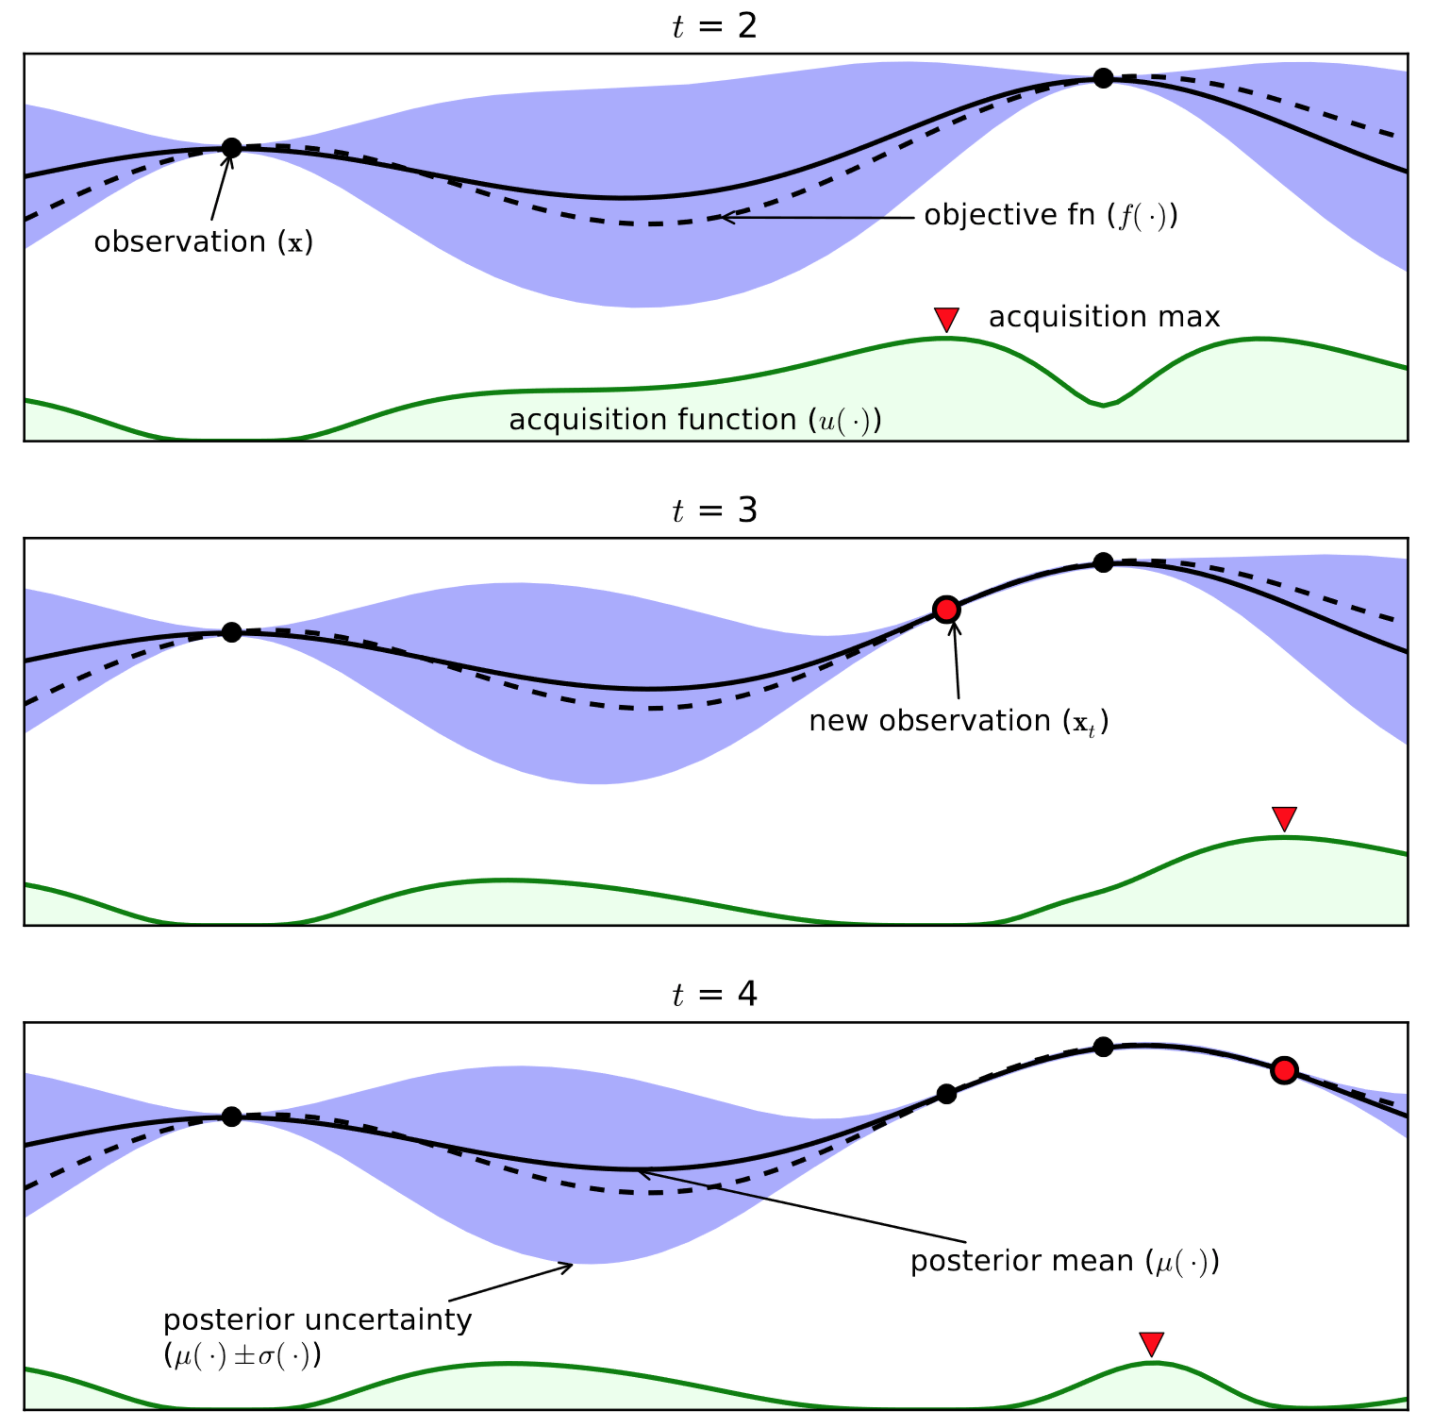
\includegraphics[width= 10cm, height = 10cm]{BOProcess.png}
	\caption{1-$d$ Bayesian Optimization Process Example~\cite{BayesianOptimizationImage}}
	\label{fig:BoProcess}
\end{figure}

According to what said above, it is possible to summarize the Bayesian Optimization' s algorithm as follow:

\begin{algorithm} [h!]
	
	\For {$n = 1, 2, ...$}
	{select new $x\textsubscript{n+1}$ by optimizing acquisition function $\alpha$ \\
		
		\begin{center}
			$x\textsubscript{n+1} = \arg \max_{x} \alpha(x, \mathcal{D}_n))$
		\end{center} 
	
	query objective function to obtain $y\textsubscript{n+1}$ \\
	augment data $\mathcal{D}\textsubscript{n+1} = \{\mathcal{D}_n, (x\textsubscript{n+1}, y\textsubscript{n+1})\}$ \\
	update statistical model 
	} 
	\caption{Bayesian Optimization\cite{DBLP:journals/pieee/ShahriariSWAF16}} 
	\label{BayAlgo}
\end{algorithm}

\subsection{An RL Approach To Black-Box Optimization} The first goal of this thesis is to describe an innovative RL based approach to optimization of black-box functions. A full, detailed chronicle of the development of the method presented in this chapter is described in \textbf{Appendix A}. The final product of all efforts will be described in the current section. \\

Let's consider the following scenario :

\begin{itemize}
	
	\item \textbf{Agent} : The Reinforcement Learning agent has to maximize a black-box bivariate function. The function is continuously defined over a specific bounded box domain, (i.e. search space). The agent has to complete its job having exactly $e$ epochs for each one of $E$ episodes. In each epoch the agent has a specific position in space described through the two coordinates $(x, y)$. Each time the agent makes an action, the \textit{angle} between $(x, y)$ and $(x', y')$ and the \textit{value} of the function $f(x', y')$, are computed.
	
	\item \textbf{State} : The state is represented by two lists: the first one contains the last two computed \textit{angles} and the second one contains the correspondent last two \textit{actions}.
	
	\item \textbf{Actions} : In each epoch the agent can make one of four different actions : \textit{move north}, \textit{move  south}, \textit{move east}, \textit{move west}. Each time the agent moves itself of a fixed number of $p$ pixels in one of the previously described directions. The resultant coordinates $(x', y')$, are computed as shown in algorithm \ref{algoPixel}.
	
	\begin{algorithm} [h!]
		/* knowing {\tt pixel\_X} and {\tt pixel\_Y} */\;
		/* knowing {\tt pixel\_X\_Range} and {\tt pixel\_Y\_Range} */ \;
		/* knowing the {\tt function} */\;
		
		\
		
		{\tt domain} = {\tt function.getDomain()} \;
		{\tt x\_Range} = {\tt domain.max\_X - domain.min\_X} \;
		{\tt y\_Range} = {\tt domain.max\_Y - domain.min\_Y} \;
		
		\
		
		{\tt x\_Real} = {\tt domain.min\_X} + {\tt(pixel\_X * x\_Range) / pixel\_X\_Range} \;
		{\tt y\_Real} = {\tt domain.min\_Y} + {\tt (pixel\_Y * y\_Range) / pixel\_Y\_Range} \;
		
		\
		
		\KwRet{{\tt x\_Real, y\_Real}}
		\caption{From pixels to real values} 
		\label{algoPixel}
	\end{algorithm}
	
	\item \textbf{Reward} : In the context just described, a real terminal state doesn't exist. Cause black-box functions are considered, it is not possible to specify two coordinates $(x, y)$ and the corresponding value function $z$ as maximum, that is, as the terminal state. For this reason every action of the agent is rewarded. The simulation ends after the $E$ episodes are completed.
	In each explored state a $\Delta$ computed as follow is defined: 
	
	\begin{equation}
		\Delta = f(x, y) - {\tt currentMax}
	\end{equation} 
	
	where $f(x, y)$ is the value function computed in the  \textit{current state}. Reward at each epoch is equal to $\Delta$.
	
\end{itemize}

The nature of the movement the agent can make in each epoch can be of two different types : \textit{linear movement} or \textit{parametric movement}. A linear movement can be thought as a crow flies one. In this case the structure of the function is not really considered. On the other hand, a parametric movement can be thought as a real movement over the function curves. In this case the structure of the function influences the amount of the movement really done. \\

If the movement is linear, the angle and the $\Delta$ (i.e. the movement amount) are computed as follow :

\begin{algorithm}
	/* knowing $(x, y)$ */ \;
	/* knowing $(x', y')$*/ \;
	/* {\tt movementAmount} = \textit{M} */ \;
	/* {\tt currentMax} = $\max f(x_n, y_n)$ */ \;
	
	
	\
	
	$z = f(x, y)$ \;
	$z' = f(x', y')$\;
	
	\
	
	$\delta = z' - z$ \;
	$\alpha = \arctan(\dfrac{\delta}{\tt movementAmount})$
	 
	 \
	 
	 $\Delta = $z'$ - {\tt currentMax} $
	 
	 \caption{Angle computation in linear movement case.} 
	
\end{algorithm}

This algorithm can be explained recalling some trigonometry. Let's suppose to be in a simple $2d$-case like the one represented in figure ~\ref{fig:LMComputations}.

\begin{figure} [h!]
	\centering
	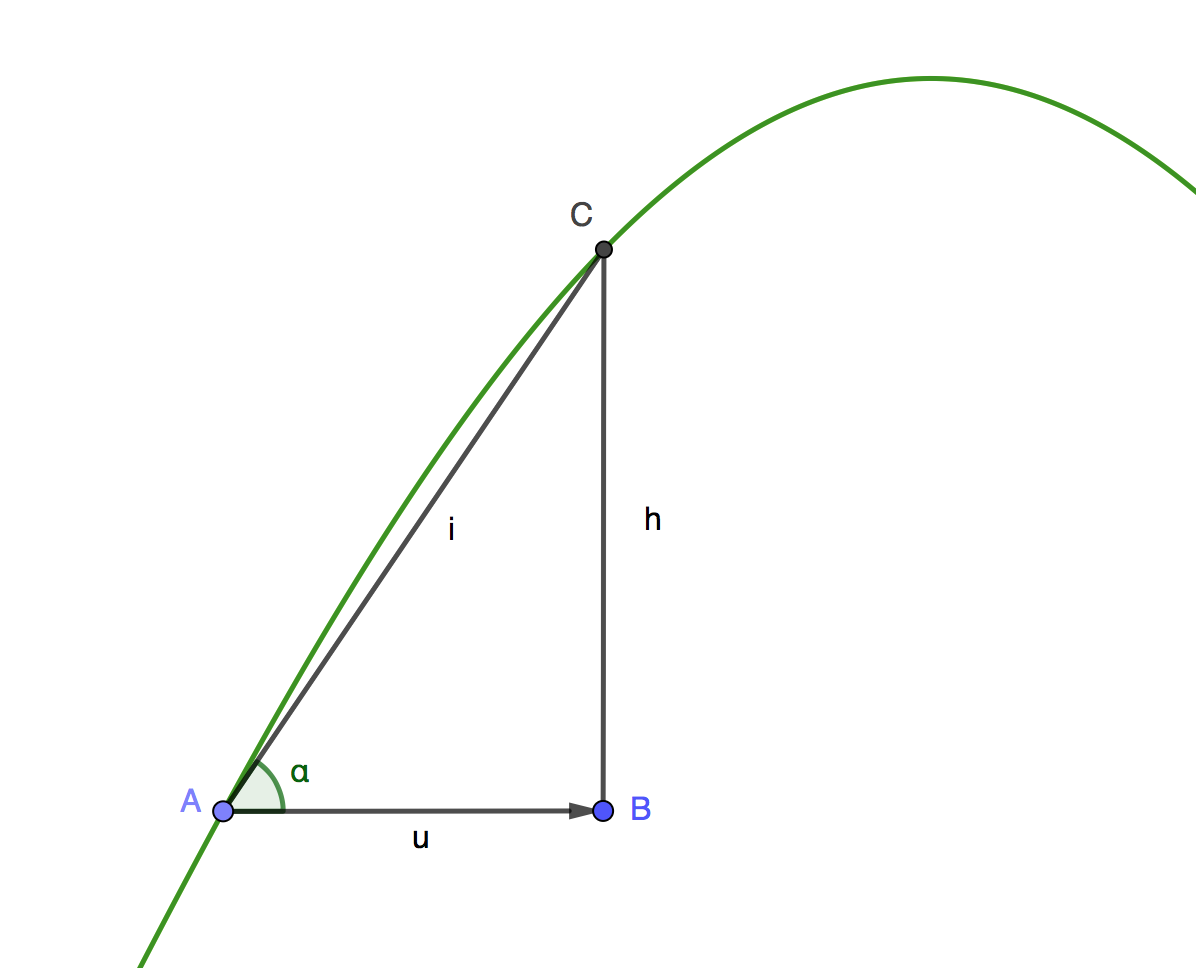
\includegraphics[width= 7cm, height = 7cm]{Triangolo.png}
	\caption{Linear movement computations.}
	\label{fig:LMComputations}
\end{figure}

Let's suppose that the starting point of the RL agent at epoch $e_i$ is the point \textit{A} with coordinates $(x, y)$. In the $1d$-case the agent can make only one of two actions for each epoch : \textit{move on} and \textit{go back}. Making a linear movement of the type \textit{move on} the arriving point at epoch $e\textsubscript{i+1}$ is \textit{B} with coordinates $(x', y)$. Knowing that the hidden objective function is $f(x) = \sin(2x)$, it is possible to compute $f(x')$. At this time point \textit{C} with coordinates $(x', f(x'))$ should be known. \textit{u} is the {\tt movement amount} and $\overline{CB}$ equals to $f(x') - f(x)$ is the $\delta$. From trigonometry 

\begin{equation}
	\tan \alpha = \dfrac{\delta}{\tt movementAmount},
\end{equation}

so it is finally possible to compute the angle $\alpha$ as follow :

\begin{equation}
	\alpha = \arctan \dfrac{\delta}{movementAmount}
\end{equation}

If the movement is parametric it is necessary to be more specific about the amount of movement over the function. This can be done using the following algorithm :

\begin{algorithm}
	/* knowing $(x, y)$ */ \;
	/* knowing $(x', y')$*/ \;
	/* {\tt movementAmount} = \textit{M} */ \;
	/* {\tt currentMax} = $\max f(x_n, y_n)$ */ \;
	
	
	\
	
	$z = f(x, y)$ \;
	$z' = f(x', y')$\;
	
	\
	
	$\delta = z' - z$ \;
	$\alpha = \arctan(\dfrac{\delta}{\tt movementAmount})$ \;
	
	\
	
	${\tt hypotenuse} = \dfrac{{\tt movementAmount}}{\cos \alpha}$ \;
	
	\
	
	${\tt projectionOnHypotenuse} = \dfrac{{\tt movementAmount} * {\tt movementAmount}}{{\tt hypotenuse}}$ \;
	
	\
	
	${\tt realMovementAmount} = {\tt projectionOnHypotenuse} * \cos \alpha$ \;
	 
	 \
	
	$\Delta = $z'$ - {\tt currentMax} $\;
	
	\caption{Computation of real movement amount in parametric movement case.} 
	\label{PMAlgo}
	
\end{algorithm}

This algorithm can be easily understood looking at figure ~\ref{fig:PMComputations}. 

\begin{figure} [h!]
	\centering
	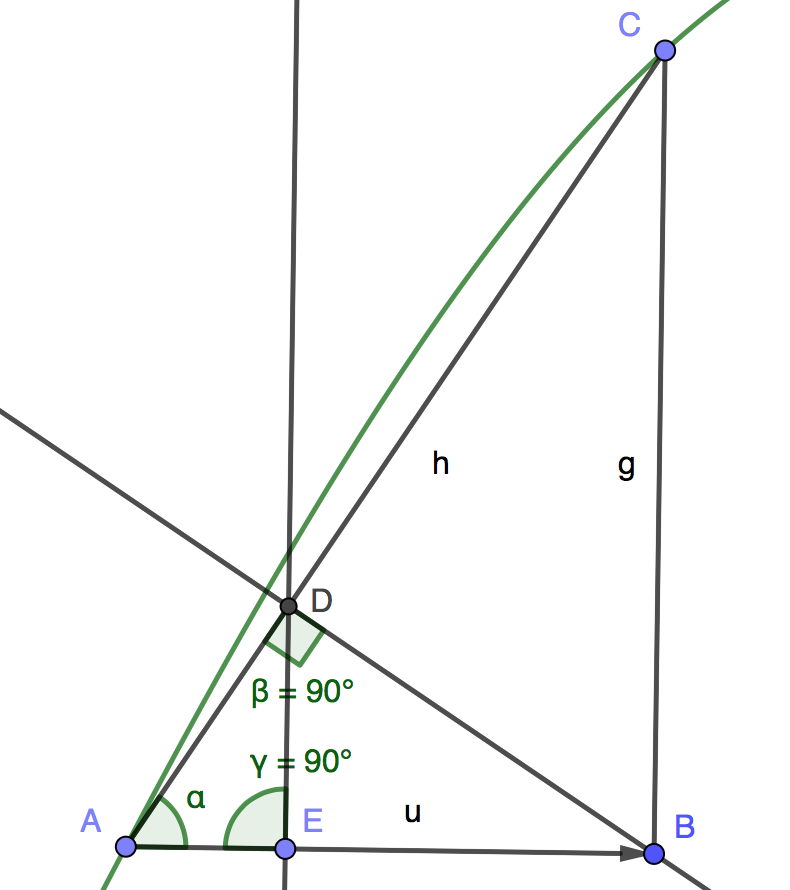
\includegraphics[width= 7cm, height = 7cm]{TRIANGOLO2.png}
	\caption{Parametric movement computations.}
	\label{fig:PMComputations}
\end{figure}

As previously done, let's suppose that the starting point of the RL agent at epoch $e_i$ is the point \textit{A} with coordinates $(x, y)$. In the case of $1d$-functions, the agent can make only one of two actions for each epoch : \textit{move on} and \textit{go back}. Making a linear movement of the type \textit{move on} the arriving point at epoch $e\textsubscript{i+1}$ is \textit{B} with coordinates $(x', y)$. Knowing that the hidden objective function is $f(x) = \sin(2x)$, it is now possible to compute $f(x')$. Point \textit{C} with coordinates $(x', f(x'))$ should now be known. \textit{u} is the {\tt movement amount} and $\overline{CB}$  equals to $f(x') - f(x)$ is $\delta$. Using trigonometry it is possible to compute $\alpha$. The goal is to know the real amount of movement done by the agent on the function. In order to do this the first thing to do is to know how much is $\overline{AE}$.  From the first theorem of Euclid it is possible to know that \textit{in a right-angled triangle, the square constructed on a cathetus is equivalent to the rectangle that has for dimensions the hypotenuse and the projection of the cathetus on the hypotenuse}. This means that in a right-angled triangle, the cathetus is proportional medium between the hypotenuse and its own projection on it. According to this it is possible to write the following proportion :

\begin{equation}
	h : u =  u : AD.
\end{equation}

So :

\begin{equation}
	AD = \dfrac{u * u}{h},
\end{equation}

that is the same of :

\begin{equation}
	 {\tt pojectionOnHypotenuse} = \dfrac{{\tt movementAmount} * {\tt movementAmount}}{{\tt hypotenuse}}
\end{equation}

of algorithm ~\ref{PMAlgo}. Now all elements useful to compute the \textit{real movement amount} represented by segment $\overline{AE}$ are known. It can be computed as follow:

\begin{equation}
	\overline{AE} = \overline{DA} \cos \alpha.
\end{equation}

Both parametric and linear approaches are effective. Therefore the question is why select one method instead of the other one. The answer to this question is simple. \\ Adopting the parametric approach the optimization process is longer but more accurate. This slowness depends on the fact that the real amount of movement is correlated with the largeness of the angle. For this reason, it is lesser at each time. 

On the other hand using the parametric approach, the agent could be ideally trained on a set of specific functions and then it should obtain better performances on a generic, never previously explored, function using its static knowledge about angles and actions, and its dynamic knowledge about function's slope. \\

Adopting the linear approach the optimization process is faster but less accurate. This depends on the fact that the movement is as the crow flies. The main difference between the linear approach and the parametric approach is that, in the first case, the slope of the function is not dynamically considered. Also in the case of the linear approach, the agent could be ideally trained on a set of specific functions, but it would obtain worse performances when this knowledge should be applied on a generic, never previously explored, function. Finally, although the set of actions available to the agent remains finite, the parametric approach enables the application of potentially infinite actions (i.e. movements), more similar to RL with \textit{parametrized actions} algorithms. Here the advantage is that the value of the action's parameter is not part of the strategy to be learned by the agent but estimated according to the knowledge acquired from the interaction with the environment.

\subsection{BURLAP Java Library}

In order to formalize and solve the problem previously described adopting an RL approach, BURLAP (Brown-UMBC Reinforcement Learning and Planning) Java library developed and maintained by James MacGlashan of Brown University, has been used. \\

BURLAP employs an highly flexible system for defining states and actions of nearly any kind of form, supporting discrete continuous, and relational domains. Planning and learning algorithms range from classic forward search planning to value function-based stochastic planning and learning algorithms~\cite{BURLAPSite}. \\

In order to define customized MDPs, BURLAP offers a set of classes and interfaces (figure ~\ref{fig:UMLBurlap}).

\begin{figure} [h!]
	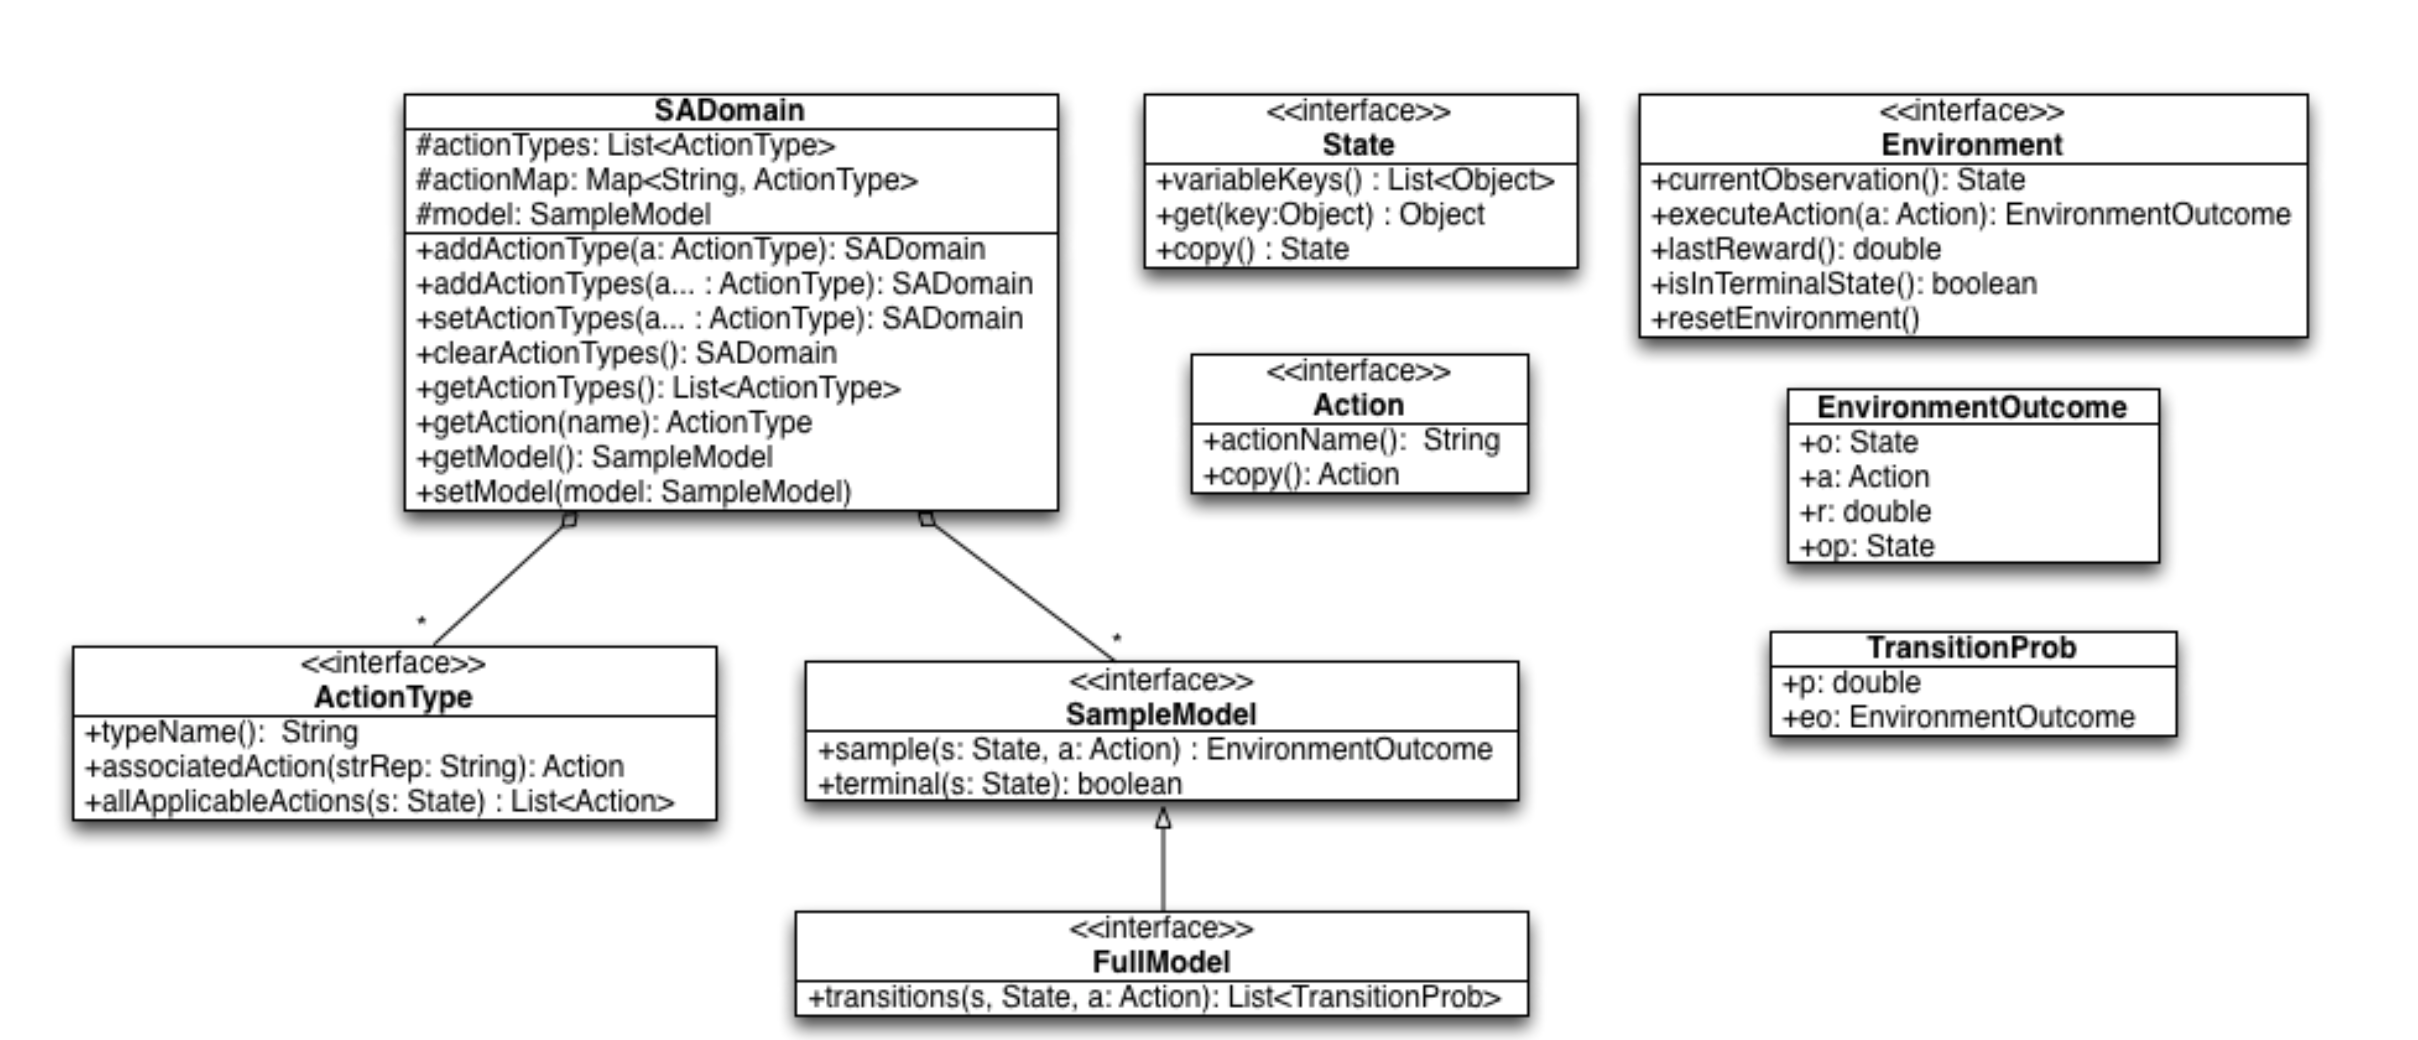
\includegraphics[width= \textwidth, height = 9cm]{UMLBurlap.png}
	\caption{UML Digram of the Java interfaces/classes for MDPs definition.}
	\label{fig:UMLBurlap}
\end{figure}

The main interfaces offered by BURLAP are :
	
\begin{itemize}
	\item \textbf{State} : implementing this interface the state variables of the MDP state space can be defined. An instance of this object specifies a single state from the states' space~\cite{BURLAPSite} .
	\item \textbf{Action} : implementing this interface a possible action that the agent can select, can be defined. If the MDP action set is discrete and unparametrized, the provided concrete implementation {\tt SimpleAction}, which defines an action entirely by a single string name, can be adopted ~\cite{BURLAPSite}.
	\item \textbf{SampleModel} : implementing this interface the model of the MDP can be defined. This interface only requires to implement methods that can sample a transition: spit back out a possible next state and reward given a prior state and action taken~\cite{BURLAPSite}.
	\item  \textbf{Environment} : An MDP defines the nature of an environment, but ultimately, an agent wants to interact with an actual environment, either through learning or to execute a policy it computed from planning for the MDP. An environment has a specific state of the world that the agent can only modify by using the MDP actions. Implementing this interface it is possible to provide an environment with which BURLAP agents can interact. If one defines a new MDP, then he will probably don't want to implement {\tt Environment} himself and instead use the provided concrete {\tt SimulatedEnvironment} class, which takes an {\tt SADomain} with a {\tt SampleModel}, and simulates an environment for its~\cite{BURLAPSite}.
\end{itemize}

An extended definition of BURLAP' s classes and interfaces can be found at \url{http://burlap.cs.brown.edu/doc/index.html}. \\

In order to model an agent able to maximize black-box functions, starting from features offered by BURLAP, interfaces and abstract classes have been implemented and extended as shown in figure ~\ref{fig:RLUMLDiagram}. \\

The full Java code can be found at this link \footnote{\url{https://github.com/AntonioBr/MIND_PROJECT}}.

\begin{figure} [h!]
	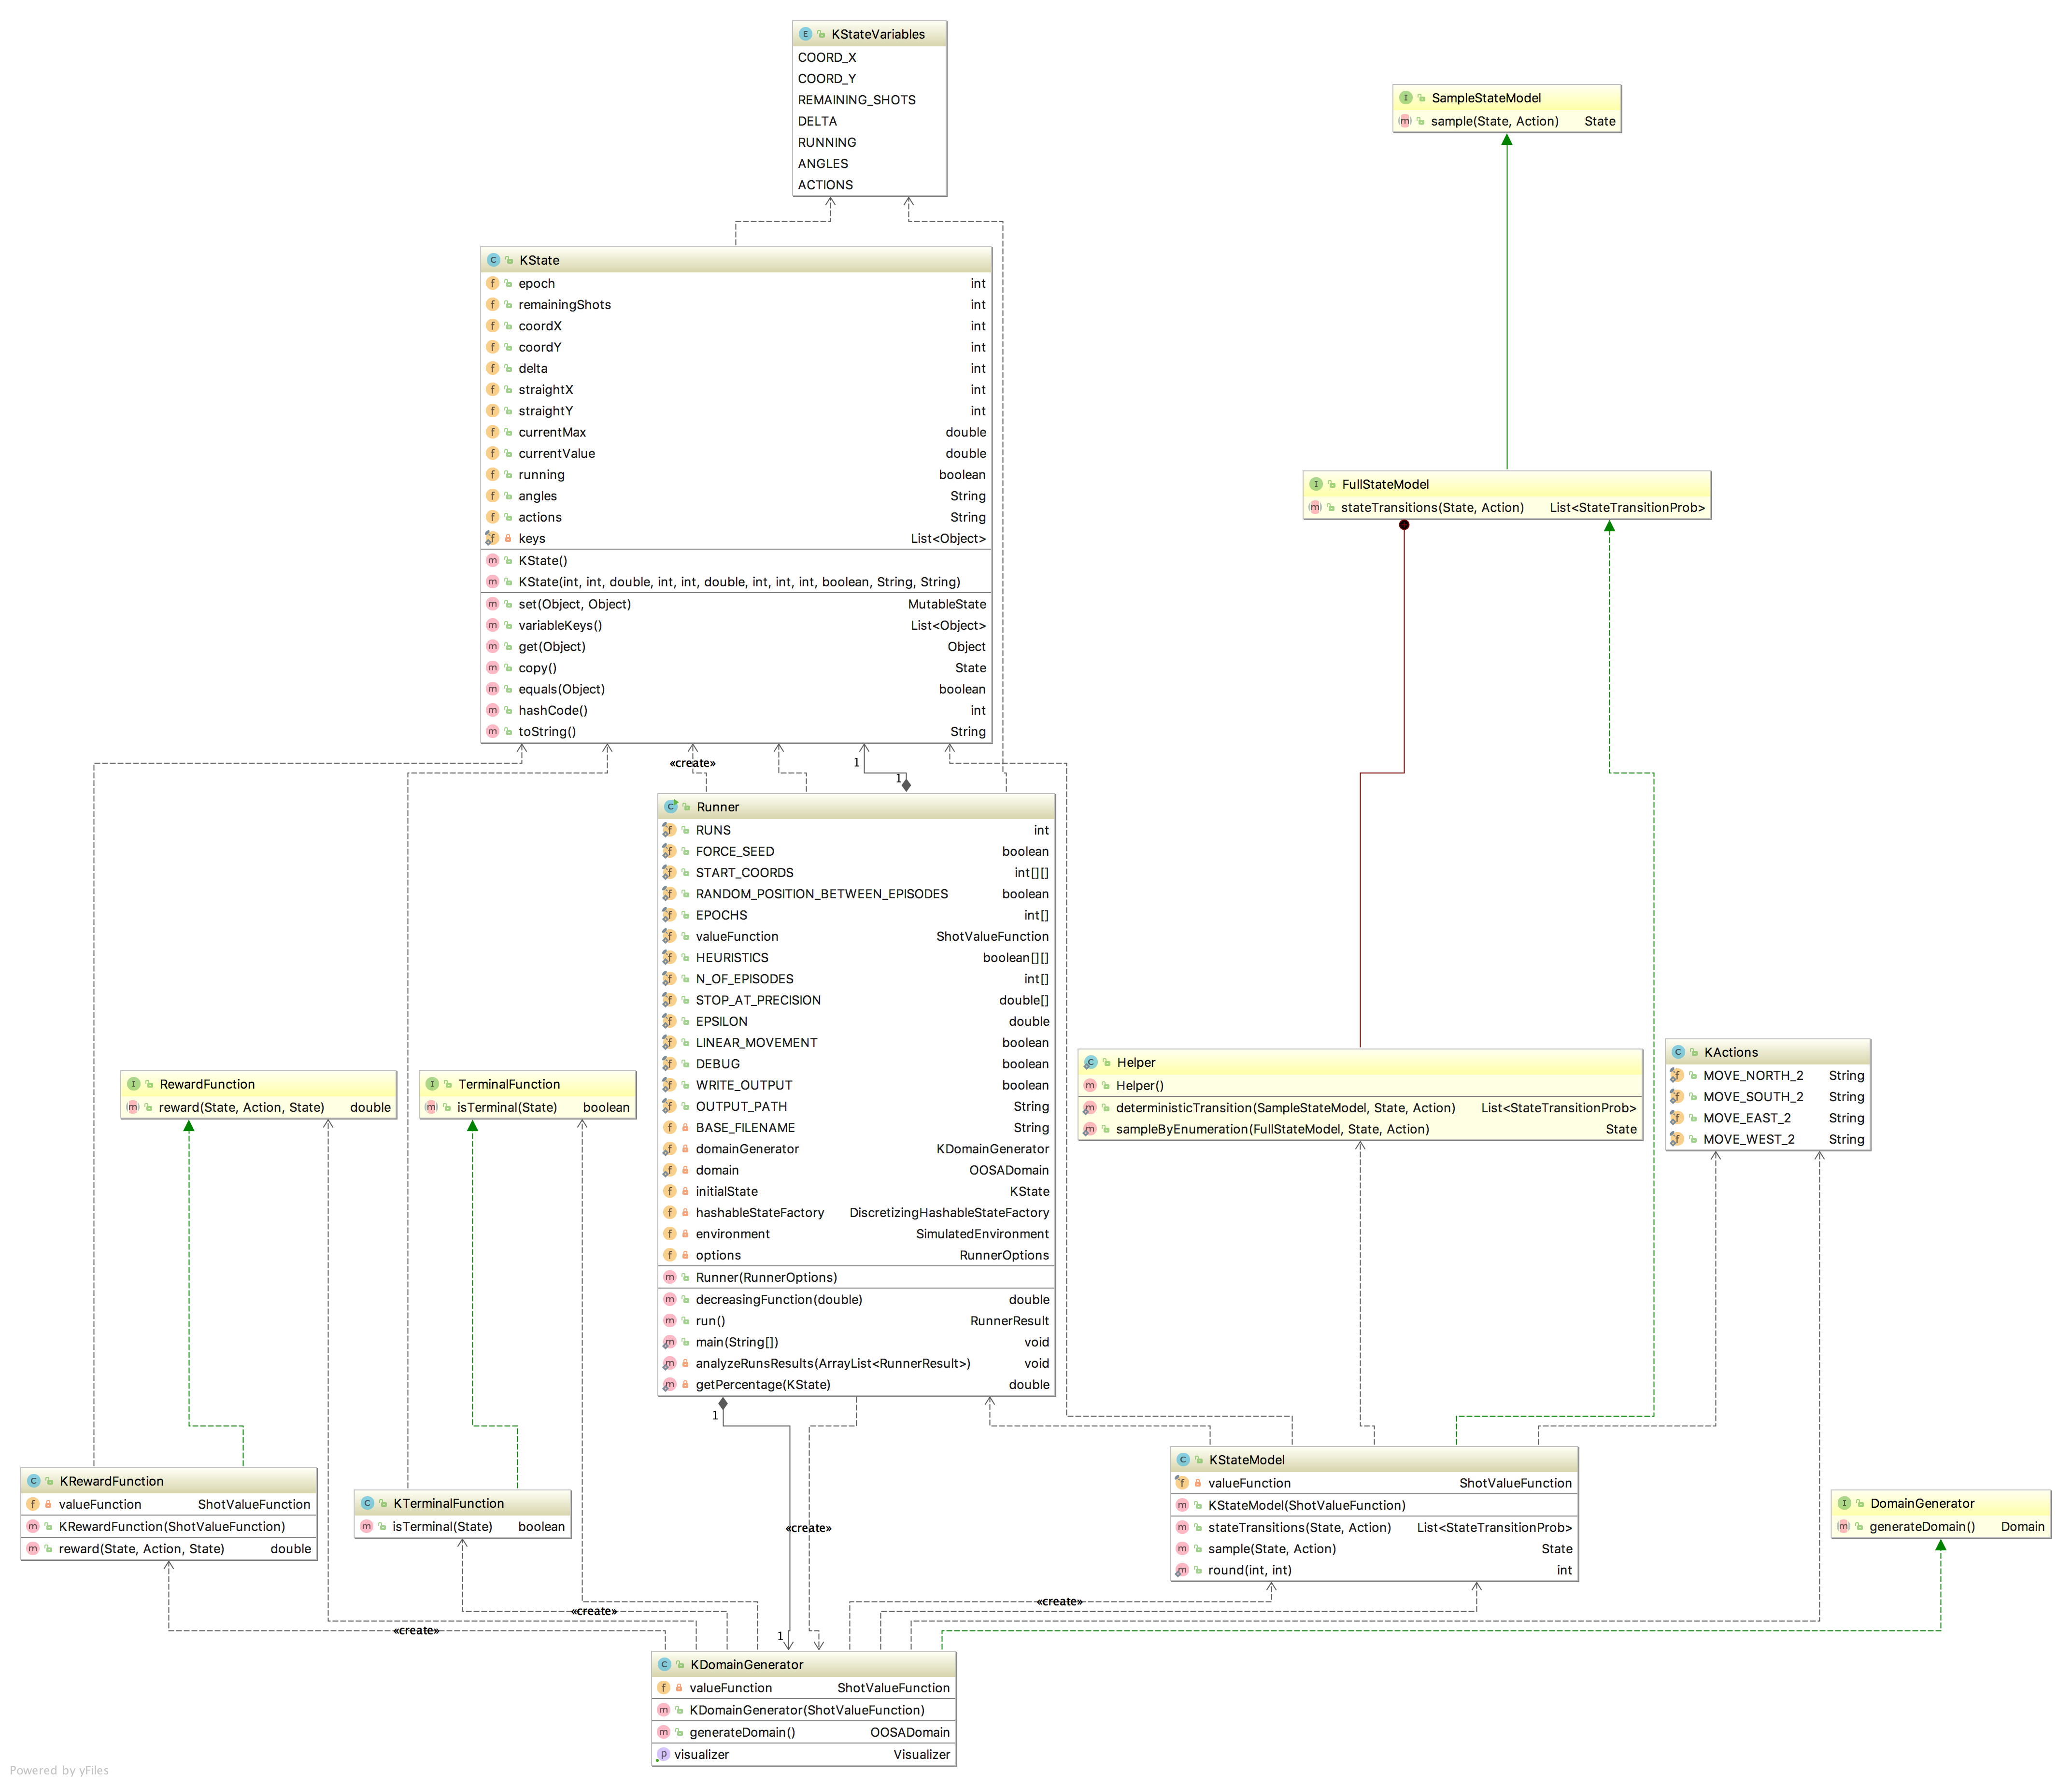
\includegraphics[width= 13cm , height = 9cm]{RLDiagram}
	\caption{Class diagram of RL based optimization approach.}
	\label{fig:RLUMLDiagram}
\end{figure}

\subsection{Humans in the Loop} Every time one gets into a rental car, he/she have to learn how hard to press the gas pedal for a given amount of acceleration. Solving this problem requires learning a relationship between two continuous variables. Over the past 50 years, several studies of \textit{function learning} have shed light on how people come to understand continuous relationships (Carroll 1963; Brehmer 1971; 1974; Koh and Meyer 1991; Busemeyer et al. 1997; DeLosh et al. 1997; Kalish et al. 2004; McDaniel and Busemeyer 2005). It has become clear that people can learn and recall a wide variety of relationships, but demonstrate certain systematic biases that tell about the mental representations and implicit assumptions that humans employ when solving function learning problems. Several models have been developed to understand the cognitive mechanisms behind function learning. Those models tend to fall into two different theoretical camps. The first includes \textit{rule-based} theories (e.g., Carroll, 1963, Brehmer, 1974, Koh and Meyer, 1991), which suggest that people learn an explicit function from a given family, such as polynomials (Carroll 1963; McDaniel and Busemeyer 2005) or power-law functions (Koh and Meyer 1991). This approach attributes rich representations to human learners, but has traditionally given limited treatment to how such representations could be acquired. A second approach includes \textit{similarity-based} theories (e.g., DeLosh et al., 1997, Busemeyer et al., 1997), which focus on the idea that people learn by forming associations: if $x$ is used to predict $y$, observations with similar $x$ values should also have similar $y$ values. Most recently, hybrids of these two approaches have been proposed (e.g., Kalish et al., 2004, McDaniel and Busemeyer, 2005), with an associative learning process that acts on explicitly represented functions. Almost all past research on computational models of function learning has been oriented towards understanding the psychological processes that underlie human performance, or the steps by which people update and deploy their mental representations of continuous relationships \cite{Lucas2015}. In this thesis, a different approach is taken, presenting a rational analysis of function learning. \\

It was seen that Bayesian Optimization applied to Gaussian Processes is a powerful tool to model, explore, and exploit unknown functions. However, it might also be applied in a different, more psychological context, namely as a model of human cognition in general and function learning in particular. Recently, Lucas, Giffiths, Williams, and Kalish (2015) have proposed also to use Gaussian Process regression as a rational model of function learning that can explain various effects within the literature of human function learning. Within the exploration-exploitation context, Borji and Itti (2013) and Wu, Schultz, Speekenbrink, Nelson, and Meder (2017) showed that Gaussian Process-based optimization can explain how participants actively search for the best output when trying to optimize one dimensional functions \cite{Schulz095190}.\\

In the next few chapters, an experiment about $2d$-function learning will be presented. The problem will be analysed from a mathematical perspective. After that, human learning techniques' performances will be compared to RL agent's ones. 